\documentclass[11pt,a4paper]{article}
\usepackage{fontspec}
\setmainfont{DejaVu Serif}
\usepackage{amsmath,amssymb,graphicx,booktabs,geometry,hyperref}
\geometry{margin=22mm}
\sloppy
\setlength{\emergencystretch}{3em}
\graphicspath{{results/}}
\begin{document}
\title{Експеримент 1: формула, гладкість і відтворення}\author{}\date{27 жовтня 2026}\maketitle

\section*{Відновлення з першоджерела}
Безпосередньо прочитано WMF-зображення рівнянь (2)--(5) у файлі
\path{pseudo_gaussian_grid_ric_formatted (2).docx} у папці авторської статті.
Їх PNG-копії збережено в \texttt{source/}. Отримуємо
\[
 \phi_{n,r}(s)=\begin{cases}(1-s^2/r^2)^{n+1},& |s|<r,\\0,&|s|\ge r,\end{cases}
 \qquad n\ge1.
\]
Коефіцієнти чотирьох наведених поліномів: $(1,-2,1)$,
$(1,-3,3,-1)$, $(1,-4,6,-4,1)$, $(1,-5,10,-10,5,-1)$.
Таким чином степінь дорівнює $2(n+1)$. Фраза $2(n+2)$ в описі
не узгоджується з цими формулами; реалізація слідує рівнянням.
Нуль у $s=r$ має кратність $n+1$, отже ядро належить $C^n$, але
не $C^{n+1}$ на межі підтримки. У центрі радіальне продовження є
поліномом від квадрата норми й не має сингулярності.
Гладкість поля сама по собі не гарантує регулярності поверхні: потрібен ненульовий градієнт.

\section*{Постановка}
\[
 f(x)=\sum_j a_j\phi_{n,r}(\|x-c_j\|),\quad
 A_{ij}=\phi_{n,r}(\|y_i-c_j\|),\quad Aa=b.
\]
Центри --- регулярна сітка. Вузли $y_i$ можуть бути зміщені від центрів
на фіксовану довжину з псевдовипадковим напрямом, seed $=0$.
Оцінюється область $[-1,1]^D$; запас означає продовження центрів
щонайменше на $r$ у кожному напрямі. Це зменшує обрізання підтримок,
але не є математичною граничною умовою чи гарантією точності.
Скінченна сума нульова поза всіма підтримками, тому її не слід
використовувати як глобальну SDF без продовження.

Для $D=2$, $h=0.25$, $n=2$ перевірено $b=1$ і
$b(x)=1+0.3x_1-0.2x_2$ на незалежній сітці $61^2$.
Чисельний ранг визначається повною SVD з порогом
$N\epsilon_{\rm machine}\sigma_{\max}$. Нульовий залишок у вузлах
не означає відтворення між ними.
\begin{center}\small\resizebox{\linewidth}{!}{\begin{tabular}{lllllll}\toprule
$r/h$ & Запас & $N$ & Ранг & $\kappa_2(A)$ & $E_1$ & $E_{\rm affine}$\\\midrule
1 & False & 81 & 81 & 1 & 0.4934 & 0.7113\\
1 & True & 121 & 121 & 1 & 0.4934 & 0.7113\\
1.5 & False & 81 & 81 & 4.699 & 0.2624 & 0.3938\\
1.5 & True & 169 & 169 & 4.974 & 0.113 & 0.1631\\
2 & False & 81 & 81 & 161.8 & 0.1389 & 0.2166\\
2 & True & 169 & 169 & 579 & 0.07441 & 0.08898\\
3 & False & 81 & 81 & 1829 & 0.05135 & 0.08379\\
3 & True & 225 & 225 & 1.823e+05 & 0.1314 & 9.132\\
\bottomrule\end{tabular}}\end{center}
Таблиця показує вибіркові максимуми похибки, а не доведені норми.
Навіть повний ранг і малий вузловий залишок не дають автоматичного
відтворення константи чи афінної функції. Покриття перевірено за
наявністю хоча б одного строго ненульового ядра в кожній точці оцінки;
це необхідна, але недостатня умова стійкості.
\begin{center}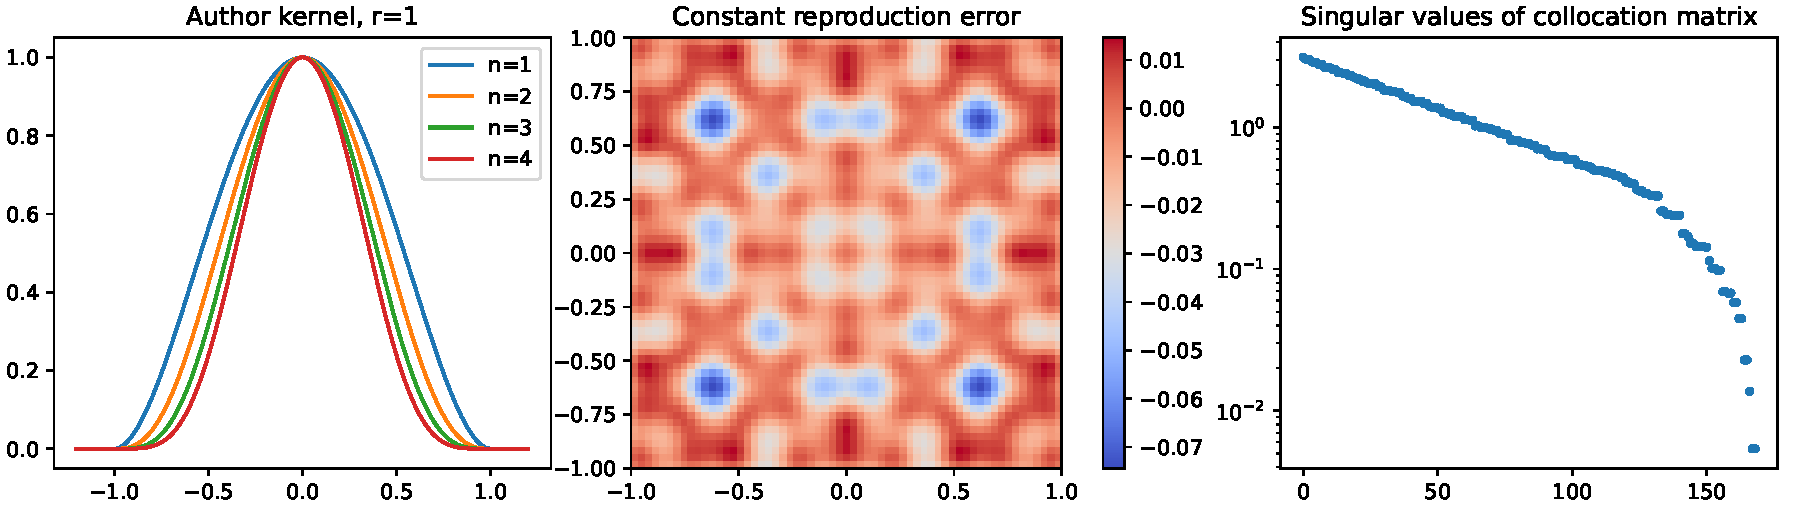
\includegraphics[width=\linewidth]{results/experiment1.pdf}\end{center}

\end{document}
